\documentclass[12pt]{extarticle}

\usepackage{preamble}

\title{Mathematical Analysis 2 Notes, Partial 2}
\date{Semester 2, 2023/2024}

\setlength{\headheight}{15pt} % ??? we do what fancyhdr tells us to do

\begin{document}

\maketitle
\tableofcontents
\clearpage

% Class of 21/03/2024
\section{Rotational Dynamics}

\subsection{Introduction}

We define a \emph{rigid body} as an object that never changes its shape.
Mathematically we can say that given any $i, j$ inside the body, the distance $d_{ij}$ will stay constant no matter what.

\subsubsection{Types of rigid bodies}

We can differentiate between continuos rigid body and discrete rigid bodies:
\begin{itemize}
    \item Continuous rigid bodies have a density mass function of the form $\rho(\vec{r})$.
    \item Discrete rigid bodies have a finite number of particles, each with a mass $m_i$ and a position $\vec{r}_i$, which might all be connected by some massless structure.
\end{itemize}

\subsubsection{Decomposing displacements}

We want to describe the motion of a rigid body in space. This is usually a hard task.

It turns out that a general displacement of a rigid body can be decomposed into the sum of two motions: a \textbf{translation} of the center of mass and a \textbf{rotation} around the center of mass.
This means that we need 6 parameters to describe any displacement: 3 for the translation and 3 for the rotation.

\subsubsection{The simplest case: 2D}

The simplest case we will consider is a 2D rigid body that lies on the $xy$ plane and can rotate around the $z$ axis.

\subsection{Angular variables}

Consider a simple case of a 2D rigid body that can rotate around the $z$ axis and has its center of mass fixed at the origin.

In this case we can describe the position of any point $p$ in the RB in polar coordinates as $(r, \theta)$. Now, knowing $r$ and $\theta$ we can compute the \textbf{arc length} $s = r\theta$.

Note that specifying $\theta$ is enough to get the position of all the points in the RB because $r$ will stay constant.

\subsubsection{Angular velocity}

Let $\omega_{\text{avg}} \coloneq \frac{\theta(t_2) - \theta(t_1)}{t_2 - t_1}$ be the \textbf{average angular velocity} between times $t_1$ and $t_2$. As $\Delta t = t_2 - t_1 \to 0$, we define the \textbf{instantaneous angular velocity} as

$$
    \omega \coloneq \lim_{\Delta t \to 0} \omega_{\text{avg}} = \dv{\theta}{t}
$$

The angular velocity is a vector, therefore we can decompose it in direction and magnitude. We have $\vec{\omega} = \omega \hat{\omega}$, where $\hat{\omega}$ is either $\hat{z}$ if the motion is counterclockwise or $-\hat{z}$ if the motion is clockwise.

Moreover note that the angular velocity stays constant for every point in the RB, but the linear velocity does not, in fact $v = r\omega$.

\subsubsection{Angular acceleration}

We define the \textbf{average angular acceleration} as $\alpha_{\text{avg}} \coloneq \frac{\omega(t_2) - \omega(t_1)}{t_2 - t_1}$ and the \textbf{instantaneous angular acceleration} as

$$
    \alpha \coloneq \lim_{\Delta t \to 0} \alpha_{\text{avg}} = \dv{\omega}{t} = \dv[2]{\theta}{t}
$$

If we want to calculate the linear acceleration of a point in the RB, we have to combine the centripetal acceleration and the tangential acceleration, that is

$$
    a = \begin{cases}
        a_c = \frac{v^2}{r} = r\omega^2 \\
        a_t = \dv{v}{t} = \dv{t}(\omega r) = r \dv{\omega}{t} = r\alpha
    \end{cases}
$$

\subsection{Rotational kinetic energy}

First we will consider a simpler case of a discrete rigid body of $n$ masses connected by a stick around a pivot which also happens to be the center of mass.

Then the kinetic energy $K = \sum_{i=1}^n K_i$ where

\begin{align*}
    K_i & = \frac{1}{2}m_i v_i^2          \\
        & = \frac{1}{2}m_i r_i^2 \omega^2
\end{align*}

note that the $i$ subscript is only present in the mass and the radius, but not in the angular velocity, then we can write

\begin{align*}
    K & = \frac{1}{2} \omega^2 \sum_{i=1}^n m_i r_i^2 \\
      & = \frac{1}{2} I \omega^2
\end{align*}

where $I \coloneq \sum_{i=1}^n m_i r_i^2$ is the \textbf{moment of inertia} of the rigid body.

\subsubsection{Moment of inertia}

We can make some trivial observations about the moment of inertia:

\begin{itemize}
    \item It depends on $m_i$ and $r_i$: if the RB is heavier or more spread out, the moment of inertia will be bigger.
    \item It depends on the axis of rotation: if we change the pivot point the moment of inertia will change because the $r_i$ will change.
\end{itemize}

In the case of a continuous rigid body, we can see it just as a sum of an infinite number of masses, so we can write

\begin{align*}
    K & = \int_{RB} \dd{K}                          \\
      & = \int_{RB} \frac{1}{2} v^2 \dd{m}          \\
      & = \int_{RB} \frac{1}{2} r^2 \omega^2 \dd{m} \\
      & = \frac{1}{2} I \omega^2
\end{align*}

where

$$
    I \coloneq \int_{RB} r^2 \dd{m} = \int_{RB} r^2 \sigma \dd{S}
$$

where $\sigma$ is the density mass function on a surface.

Note that $r$ and $\sigma$ are functions of the position, even if we dropped the notation this does not mean that $I$ is a constant.

\begin{remark}
    For a matter of notation, we will use the symbol $\lambda$ to denote the linear density mass function, $\sigma$ to denote the surface density mass function and $\rho$ to denote the volume density mass function.
\end{remark}

\begin{example}[moment of inertia of a ring]
    Consider a ring of radius $R$ and mass $M$ with uniform density. We want to calculate the moment of inertia with respect to the center of the ring.

    Since the density is uniform, we can write $\lambda = \frac{M}{2\pi R}$, then

    \begin{align*}
        I & = \int_{\text{ring}} r^2 \dd{m}         \\
          & = \int_{\text{ring}} R^2 \lambda \dd{r} \\
          & =  R^2 \int_{\text{ring}} \dd{m}        \\
          & = R^2 M
    \end{align*}
\end{example}

\begin{example}[moment of inertia of a disk]
    Consider a disk of radius $R$ and mass $M$ with uniform density. We want to calculate the moment of inertia with respect to the center of the disk.

    Since the density is uniform, we can write $\sigma = \frac{M}{\pi R^2}$.

    We have two ways to compute $I$. The first one is to brute force the definition of $I$, passing to polar coordinates and solving the integral.

    With this method we get that $\dd{S} = r \dd{r} \dd{\theta}$, then

    \begin{align*}
        I & = \int r^2 \dd{m} = \int r^2 \sigma \dd{S}             \\
          & = \int r^2 \sigma r \dd{r} \dd{\theta}                 \\
          & = \sigma \int_0^{2\pi} \dd{\theta} \int_0^R r^3 \dd{r} \\
          & = 2 \pi \sigma \frac{R^4}{4} = \frac{1}{2} M R^2
    \end{align*}

    Alternatively we can sum the moment of inertia of a ring of radius $r$ and width $\dd{r}$ and use the result we got in the previous example.
    We have

    \begin{align*}
        I & = \int \dd{I_\text{ring}} = \int r^2 \dd{m_\text{ring}}             \\
          & = \int r^2 \sigma \dd{S_\text{ring}}= \int r^2 \sigma 2\pi r \dd{r} \\
          & = 2\pi \sigma \int r^3 \dd{r} = 2\pi \sigma \frac{R^4}{4}           \\
    \end{align*}

    which indeed is the same result as before at the expense of a much simpler integral.
\end{example}

% Class of 25/03/2024

\begin{example}(moment of inertia of a rod)
    Consider a rod of length $L$ and mass $M$ with density mass function $\lambda = \frac{M}{L} = \text{const}$.

    If we calculate the moment of inertia at the point $x = 0$ we get

    $$
        I_0 = \int_0^L x^2 \dd{m} = \int_0^L x^2 \lambda \dd{x} = \left[ \lambda frac{x^3}{3} \right]_0^L = \frac{1}{3} ML^2
    $$

    Note that the moment of inertia depends on the point we calculate it on, for instance, if we calculate it at the center of mass we get

    $$
        I_{\text{cm}} = \int_{-L/2}^{L/2} x^2 \lambda \dd{m} = \left[ \lambda \frac{x^3}{3} \right]_{-L/2}^{L/2} = \frac{1}{12} ML^2
    $$

    that is, $I_0 > I_{\text{cm}}$, in particular, $I_0 = I_{\text{cm}} + M \left(\frac{L}{2}\right)^2$.
    We note that $L/2$ is the distance between the two points, so can think about generalizing this result to any two points, which is what we are going to do in the next section.
\end{example}

\subsection{Parallel axis theorem}

Before staring with the theorem, we need this remark:
\begin{remark}
    Let $\vec{A}, \vec{B}$, then
    $$
        \left( \vec{A} + \vec{B} \right) \cdot \left( \vec{A} + \vec{B} \right) = \abs{\vec{A} + \vec{B}}^2 = A^2 + 2 \vec{A} \cdot \vec{B} + B^2
    $$
\end{remark}

\begin{theorem}[parallel axis theorem]
    Consider a rigid body with moment of inertia $I_{\text{cm}}$ with respect to the center of mass and mass $M$. Then the moment of inertia $I$ with respect to any other point $O$ at a distance $d$ from the center of mass is

    $$
        I_O = I_{\text{cm}} + M d^2
    $$

    \label{thm:parallel_axis}
\end{theorem}

\begin{proof}
    We have that $I_O = \sum^N m_i r_i^2$, then let $\vec{d}$ be the distance between the center of mass and $O$, $\vec{r'}_i$ be the distance between the center of mass and $i$ and $\vec{r}_i$ be the distance between $O$ and $i$.

    Then $\vec{r}_i = \vec{r'}_i + \vec{d}$, so we can write

    $$
        (\vec{r}_i)^2 = \abs{\vec{r'}_i + \vec{d}}^2 = (\vec{r'}_i)^2 + 2 \vec{r'}_i \cdot \vec{d} + (\vec{d})^2 = (r_i')^2 + d^2 + 2 \vec{r'}_i \cdot \vec{d}
    $$

    We want to write the moment of inertia as

    \begin{align*}
        I_O & = \sum^N_{i = 1} m_i r_i^2 = \sum^N_{i = 1} m_i (r_i')^2 + \sum^N_{i = 1} m_i d^2 + 2 \sum^N_{i = 1} m_i \vec{r'}_i \cdot \vec{d} \\
            & = \sum^N_{i = 1} m_i (r_i')^2 + M d^2 + 2 \vec{d} \cdot \sum^N_{i = 1} m_i \vec{r'}_i
    \end{align*}

    and in order to prove the theorem we need to show that the last term is zero.
    Indeed we have that
    $$
        \sum^N_{i = 1} m_i \vec{r'}_i = M \vec{r}_{\text{cm}} = 0
    $$
    because the center of mass is the origin of the reference frame of the $r_i'$.
\end{proof}

This is very useful to compute the kinetic energy of a rigid body that is rotating around a point that is not the center of mass.
We have that

\begin{align*}
    K & = \frac{1}{2} I_O \omega^2                                           \\
      & = \frac{1}{2} (I_{\text{cm}} + M d^2) \omega^2                       \\
      & = \frac{1}{2} I_{\text{cm}} \omega^2 + \frac{1}{2} M (d \omega)^2    \\
      & = \frac{1}{2} I_{\text{cm}} \omega^2 + \frac{1}{2} M v_{\text{cm}}^2
\end{align*}

\subsection{Torque}

Torque is the equivalent of force in rotational dynamics. It is defined as

\begin{align*}
    \vec{\tau} & \coloneq \vec{r} \times \vec{F} \\
               & = r F \sin(\theta)              \\
               & = r F_t
\end{align*}

where $F_t$ is the tangential component of the force.
Note that $\tau > 0$ if the rotation it causes is counterclockwise.

\subsubsection{Newton's law for rotation}

As we said before, torque is the equivalent of force in rotational dynamics. Then

\begin{theorem}
    $$
        \tau = I \alpha
    $$
\end{theorem}

\begin{proof}
    We have that $F_t = F \sin \theta = m a_t$, but $a_t$ can be written in terms of the angular acceleration, so we can write $F_t = m r \alpha$.

    Now if we multiply both sides by $r$

    \begin{align*}
        r F_t & = m r^2 \alpha \\
        \tau  & = I \alpha
    \end{align*}
\end{proof}

This works even if there are multiple forces actin on multiple points:
\begin{itemize}
    \item If there are multiple forces acting on a singular point we can just sum the forces to obtain the total torque.
    \item If we have multiple forces acting on multiple points we can sum the torques of each force acting on each point and then sum all the torques.
\end{itemize}

Even though these could look like two different cases, they are actually the same thing:

$$
    \tau = \sum_i \tau_i = \sum_i m_i r_i^2 \alpha = \alpha \sum_i m_i r_i^2 = I \alpha
$$

that is because $\alpha$ is the same for all the points in the rigid body.

Moreover, if we define the \emph{angular momentum} as
$$
    L \coloneq I \omega
$$

we can write Newton's law for rotation as

$$
    \tau = I \alpha = I \dv{\omega}{t} = \dv{L}{t}
$$

\subsubsection{Torque due to gravity}

If we have a rigid body with mass $M$ and center of mass at the origin, we can calculate the torque due to gravity as the integral of the torque due to the force of gravity acting on each point of the rigid body.

$$
    \dd{\tau} = \dd{F} r \sin \theta = \dd{m} g r \sin \theta = \dd{m} g r_x
$$

Then

$$
    \tau = \int_{RB} \dd{\tau} = \int_{RB} \dd{m} g r_x = g \int_{RB} \dd{m} r_x = M g x_{\text{cm}}
$$

\subsubsection{Work}

We know by the definition of work that $\dd{W} = F \cdot \dd{s}$. In the case of torque we have that the radial component of the force is \say{useless} and doesn't produce any work. Then

$$
    \dd{W} = F_t \dd{s} = F_t r \dd{\theta} = \tau \dd{\theta}
$$

\subsection{Summary table}

We can keep track of the variables we have defined in a table.

\begin{table}[H]
    \centering
    \begin{tabular}{|c|c|c|}
        \hline
        \textbf{Variable} & \textbf{1D}             & \textbf{2D rotation}         \\
        \hline
        Position          & $x$                     & $\theta$                     \\
        Velocity          & $v = \dv{x}{t}$         & $\omega = \dv{\theta}{t}$    \\
        Acceleration      & $a = \dv[2]{x}{t}$      & $\alpha = \dv[2]{\theta}{t}$ \\
        Inertia           & $m$                     & $I$                          \\
        Force/Torque      & $F = ma$                & $\tau = I \alpha$            \\
        Momentum          & $p = mv$                & $L = I \omega$               \\
        Kinetic energy    & $K = \frac{1}{2} m v^2$ & $K = \frac{1}{2} I \omega^2$ \\
        Work              & $\dd{W} = F \dd{x}$     & $\dd{W} = \tau \dd{\theta}$  \\
        \hline
    \end{tabular}
    \caption{Summary of angular variables}
    \label{tab:angular-variables}
\end{table}

and if $\alpha = \text{const}$ we have

$$
    \begin{cases}
        \theta(t) & = \theta_0 + \omega_0 t + \frac{1}{2}\alpha t^2 \\
        \omega(t) & = \omega_0 + \alpha t
    \end{cases}
$$


\subsection{Translation and rotation}

We are interested in the motion of a rigid body that is both rotating and translating, for example a wheel.

We will consider only the case in which the wheel is rolling without slipping, that is, after a full rotation the wheel has moved of a distance equal to its circumference.
We can express this condition as follows:

$$
    s_{\text{cm}} = R \theta
$$
or, let $f$ be the frequency of the rotation, then the velocity of the center of mass is
$$
    v_{\text{cm}} = 2 \pi R f = \omega R
$$

\begin{figure}[H]
    \centering
    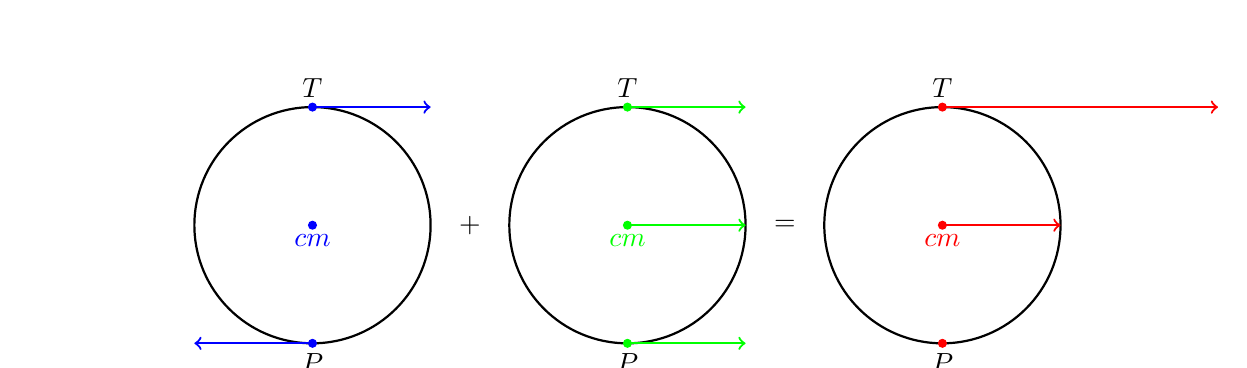
\begin{tikzpicture}
        \node at (-7.5, 0) {};

        \draw[thick] (-4, 0) circle (1.5);
        \draw[thick, ->, blue] (-4, 1.5) -- (-2.5, 1.5);
        \filldraw[blue] (-4, 1.5) circle (0.05);
        \node[anchor=south] at (-4, 1.5) {$T$};

        \filldraw[blue] (-4, 0) circle (0.05) node[anchor=north] {$cm$};

        \draw[thick, ->, blue] (-4, -1.5) -- (-5.5, -1.5);
        \filldraw[blue] (-4, -1.5) circle (0.05);
        \node[anchor=north] at (-4, -1.5) {$P$};

        \node at (-2, 0) {$+$};

        \draw[thick] (0, 0) circle (1.5);

        \draw[thick, ->, green] (0, 1.5) -- (1.5, 1.5);
        \filldraw[green] (0, 1.5) circle (0.05);
        \node[anchor=south] at (0, 1.5) {$T$};

        \draw[thick, ->, green] (0, 0) -- (1.5, 0);
        \filldraw[green] (0, 0) circle (0.05) node[anchor=north] {$cm$};

        \draw[thick, ->, green] (0, -1.5) -- (1.5, -1.5);
        \filldraw[green] (0, -1.5) circle (0.05);
        \node[anchor=north] at (0, -1.5) {$P$};

        \node at (2, 0) {$=$};

        \draw[thick] (4, 0) circle (1.5);

        \draw[thick, ->, red] (4, 1.5) -- (7.5, 1.5);
        \filldraw[red] (4, 1.5) circle (0.05);
        \node[anchor=south] at (4, 1.5) {$T$};

        \draw[thick, ->, red] (4, 0) -- (5.5, 0);
        \filldraw[red] (4, 0) circle (0.05) node[anchor=north] {$cm$};

        \filldraw[red] (4, -1.5) circle (0.05);
        \node[anchor=north] at (4, -1.5) {$P$};
    \end{tikzpicture}

    \caption{Constructing rolling without slipping motion from pure rotation and pure translation.}
    \label{fig:rolling-without-slipping}
\end{figure}

We can obtain this kind of motion by \say{summing} a pure rotation and a pure translation:
\begin{itemize}
    \item In the pure rotation $v_{\text{cm}} = 0$, $v_{P} = - \omega R \hat x$ and $v_{T} = \omega R \hat x$.
    \item In the pure translation $v_{\text{cm}} = v_{P} = v_{T} = \omega R \hat x$.
\end{itemize}
then by summing the two motions we get that $v_{\text{cm}} = \omega R \hat x$, $v_{P} = 0$ and $v_{T} = 2 \omega R \hat x$.

We can also calculate the total kinetic energy using the parallel axis theorem \ref{thm:parallel_axis}:
\begin{align*}
    K & = \frac{1}{2} I_{\text{cm}} \omega^2 + \frac{1}{2} M v_{\text{cm}}^2 \\
      & = \frac{1}{2} M \omega^2 R^2 + \frac{1}{2} \frac{M R^2}{2} \omega^2  \\
      & = \frac{1}{2} \frac{3M R^2}{2} \omega^2                              \\
      & = \frac{1}{2} I_{\text{edge}} \omega^2
\end{align*}
where the first $I_{\text{cm}}$ is the inertia of a disk and the second $I_{\text{edge}}$ is the inertia of a disk, that is, the edge of the wheel.

This is an interesting result because it tells us that we can view the translation-rotation motion as a pure rotation motion around the point of contact $P$ between the wheel and the ground.

\subsection{Angular momentum}

We have defined the angular momentum as $L = I \omega$. We can also define the torque as $\tau = \dv{L}{t}$.

If we consider a system where $\tau = 0$ we have that since $\tau = \dv{L}{t}$ the momentum $L$ is constant.

\begin{example}
    Consider two disks with inertia $I_1$ and $I_2$ and angular velocities $\omega_1 \ne 0$ and $\omega_2 = 0$, both of them have a stick going through their centers and they are free to rotate around the stick.
    Disk 2 touches disk 1 and they start rotating together around the stick.

    We can calculate the final angular velocity $\omega$ of the system as follows:
    \begin{align*}
        I_1 \omega_1 + \cancel{I_2 \omega_2} & = (I_1 + I_2) \omega             \\
        \omega                               & = \frac{I_1 \omega_1}{I_1 + I_2}
    \end{align*}
\end{example}

\begin{example}[ice skater]
    An ice skater is spinning with her arms outstretched, then she pulls her arms in.
    We want to calculate how does her angular velocity change.

    The difference between the two positions causes the moment of inertia to change because the mass is less spread out.
    Let $I_1$ be the moment of inertia with the arms outstretched and $I_2 = \frac{1}{2} I_1$ the moment of inertia with the arms pulled in and applying the conservation of momentum we get $\omega_2 = 2 \omega_1$.

    Moreover, we can calculate the kinetic energy of the system as
    $$
        K_2 = \frac{1}{2} I_2 \omega_2^2 = \frac{1}{2} \left(\frac{1}{2} I_1\right) (2 \omega_1)^2 = 2 K_1
    $$

    This additional energy comes from the fact that the skater has to do work to pull her arms in.
\end{example}

When applying conservation of momentum choosing the right point to calculate the moment of inertia is crucial.
In fact, it is possible to have systems where the torque is zero only if we choose the right reference frame, usually choosing the center of mass as the origin of such reference frame is a good guess.

% Class of 27/03/2024

\subsection{Tensor of inertia}

\begin{figure}[H]
    \centering
    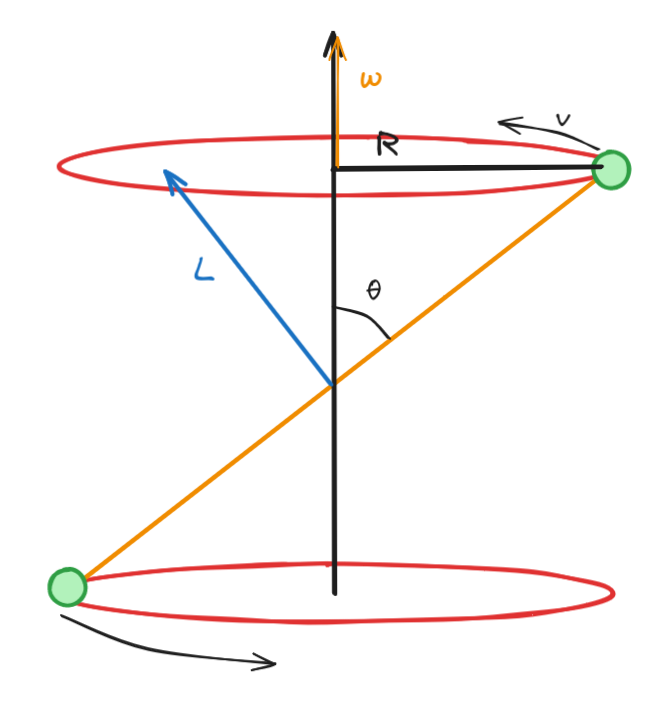
\includegraphics[width=0.5\textwidth]{assets/S2_P2_PHY1/skew.png}
    \caption{A system where the angular momentum is not parallel to the angular velocity.}
    \label{fig:tensor-of-inertia}
\end{figure}

We can write the angular velocity as $\vec{\omega} = \vec{r} \times \vec{v}$, then in this case we have $\hat \omega = \hat z$.

We can calculate the momentum as
$$
    \abs{\vec L} = \abs{\vec{L}_{\text{top}} + \vec{L}_{\text{bottom}}} = dmv = md\omega R
$$
then
\begin{align*}
    L_z & = L \cos \alpha = L \sin \theta                       \\
        & = md\omega R \sin \theta                              \\
        & = 2 m \omega R \left( \frac{d}{2} \sin \theta \right) \\
        & = 2m R^2 \omega
\end{align*}

We see that in this case $\vec{L}$ and $\vec{\omega}$ don't point in the same direction.

This is because $I$ is not just a scalar but we have to specify it for all the three directions, expressing it as a matrix:
$$
    I = \begin{pmatrix}
        I_{xx} & I_{xy} & I_{xz} \\
        I_{yx} & I_{yy} & I_{yz} \\
        I_{zx} & I_{zy} & I_{zz}
    \end{pmatrix}
$$
this matrix is symmetric, that is $I_{ij} = I_{ji}$. We call this matrix \emph{tensor of inertia}.

In order to compute the elements of the matrix it can be shown that
$$
    \begin{cases}
        I_{zz} = \sum_i m_i (x_i^2 + y_i^2) \\
        I_{yz} = - \sum_i m_i x_i y_i       \\
        I_{xz} = - \sum_i m_i x_i z_i       \\
    \end{cases}
$$
and for $\vec{L}$ we have
$$
    \vec{L} = \begin{pmatrix}
        L_x \\
        L_y \\
        L_z
    \end{pmatrix}
    =
    \begin{pmatrix}
        I_{xz} \omega \\
        I_{yz} \omega \\
        I_{zz} \omega
    \end{pmatrix}
$$

With some linear algebra sorcery (spectral theorem), it is possible to show that it is always possible to find such a reference frame where the tensor of inertia is diagonal and the angular momentum is parallel to the angular velocity for any object.
This only happens when the object is rotating around one of its principal axes (one of its axes of symmetry).

\end{document}
